\hypertarget{results}{%
	\section{Results}\label{results}}

If you're going to make adaptive management decision in terms of our perspective (interactive disturbance regime ecosystem) these are data that will support these adaptive management decisions.

\hypertarget{identification-of-current-multi-species-management-goals-and-ecological-objectives}{%
	\subsection{Identification of Current Multi-Species Management Goals and Ecological Objectives} \label{identification-of-current-multi-species-management-goals-and-ecological-objectives}}

\begin{itemize}
	\item Bison management
	\item Invasive species management
	\item Native ecosystems
\end{itemize}

\hypertarget{bison-management}{%
	\subsubsection{Bison Management}\label{bison-management}} 

Of particular importance at these NPS units is bison management. 
Four out of the five units currently have bison on site (BADL, TAPR, THRO, and WICA) and three out of four currently have a management plan written for bison (BADL, TAPR, and WICA). 
When looking at these management plans, the overall goal is the genetic viability of the herd.
Ecologically, in the BADL bison management plan, vegetation is considered, but effects on other wildlife are not.

\hypertarget{invasive-species-management}{%
\subsubsection{Invasive Species Management} \label{invasive-species-management}}

In terms of vegetation, invasive species management is the top concern.
For example, in a vegetation management strategy written for THRO, invasive species management is thoroughly discussed rather than enhancing the vigor of native populations.

\hypertarget{native-ecosystems}{%
\subsubsection{Native Ecosystems} \label{native-ecosystems}}

Our interview guide asked managers what their goals were for the ecosystem they protect. 
Typically, this goal included some aspect of
maintaining a natural ecosystem. 
The particulars of how this could be achieved were not explicit. The feeling
that we have is that there needs to be a higher level of consistency in
getting fire on the landscape. Figure 5 displays the fires history of
the five units in this study. One thing to note is although Tallgrass
has many more fires per year, which is a construct of the type of
ecosystem that TAPR protects. The fire return interval in this area of
the country is much shorter and makes fire a much more frequent
disturbance than at the other units in this study. Accordingly, TAPR has
more consistent fires compare to other units.

\begin{figure*}[th]
	\centering
	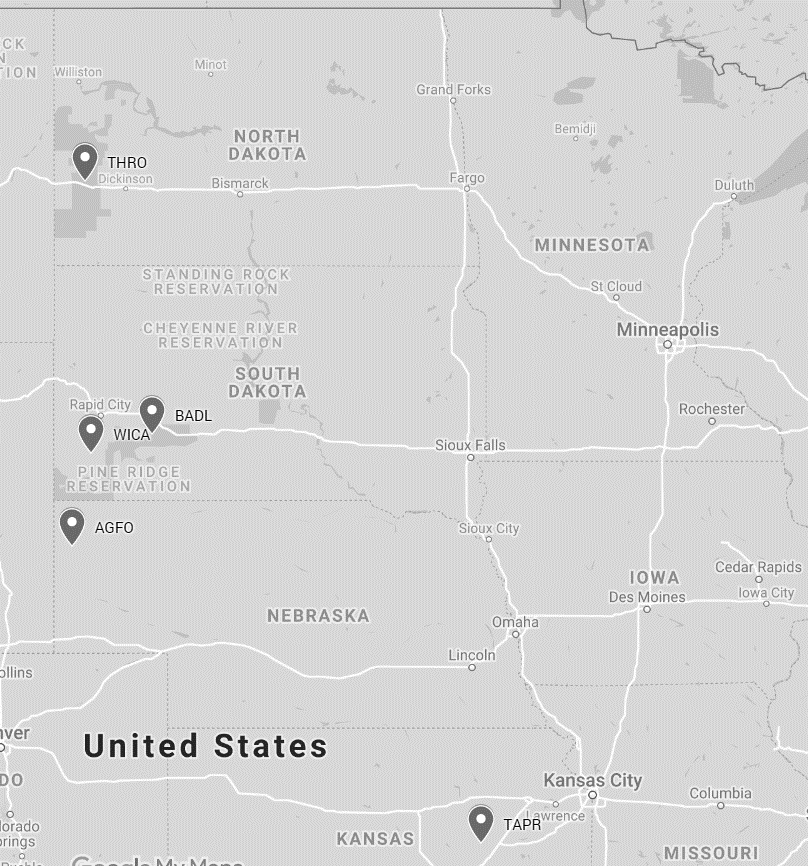
\includegraphics[width=0.75\textwidth]{figures/RegionMapGoogle.png}\caption[Rx fires in Midwest NPS units, 2008\textendash 2017.]{Prescribed fires in Midwest region NPS units 2008\textendash 2017.} \label{RxFires}
\end{figure*}

In further detail, THRO had no prescribed fire occurrence from 2012\textendash 2017. 
The fire history in THRO was rich until 2012, but 2018 saw a large fire in pursuit of impacting juniper encroachment. 
BADL has also had an inconsistent fire occurrence with no fires occurring from 2013\textendash 2015. 
Interviews revealed that this had to do somewhat with budget and staffing concerns. 
WICA and AGFO have also had periods of no fire which did not create any areas of patch contrast.

\hypertarget{recommended-management-changes}{%
\subsection{Recommended Management Changes}\label{recommended-management-changes}}

\begin{itemize}
	\item Establish coupled disturbance regimes
	\item Manage for ecosystem processes
\end{itemize}

\hypertarget{establish-coupled-disturbance-regime}{%
\subsubsection{Establish Coupled Disturbance Regime}
\label{establish-coupled-disturbance-regime}}

In order to achieve heterogeneity we suggest coupling ecosystem
disturbances. In particular it has been proven to be beneficial in that
past to couple fire and grazing into a disturbance regime. A technique
that has had success in this region is a process called patch burn
grazing. Through patch burn grazing, pastures are created with
contrasting ecosystem characteristics. Each year, one pasture is burned
and this contrast benefits wildlife, grazers, vegetation, etc. The
following year, the areas that were burned grow back with nutritive new
growth benefiting herbivores.

An example of a successful program coupling disturbances is occurring at TAPR. 
In 2006, they established a technique called patch burn grazing in one pasture at their unit. 
Patch burn grazing techniques require annual burns on different patches of the designated area \citep{fuhlendorf2009, toombs2010, scasta2016}. 
As seen in Fig.~\ref{PBGatTAPR}, the pasture has been split into three patches which are burned on an annual schedule. 
By burning on this schedule, there are heterogeneous patches benefiting native grazers and other wildlife as well as the vegetation structure of the preserve. 
As this is already occurring on an NPS unit, it makes it more plausible to instill a coupled disturbance regime on other units across the Midwest region. 
This disturbance regime has benefitted TAPR in many ways
and I\&M monitoring data has showed\ldots{} \citep{leis2018}.

\begin{figure*}[th]
	\centering
	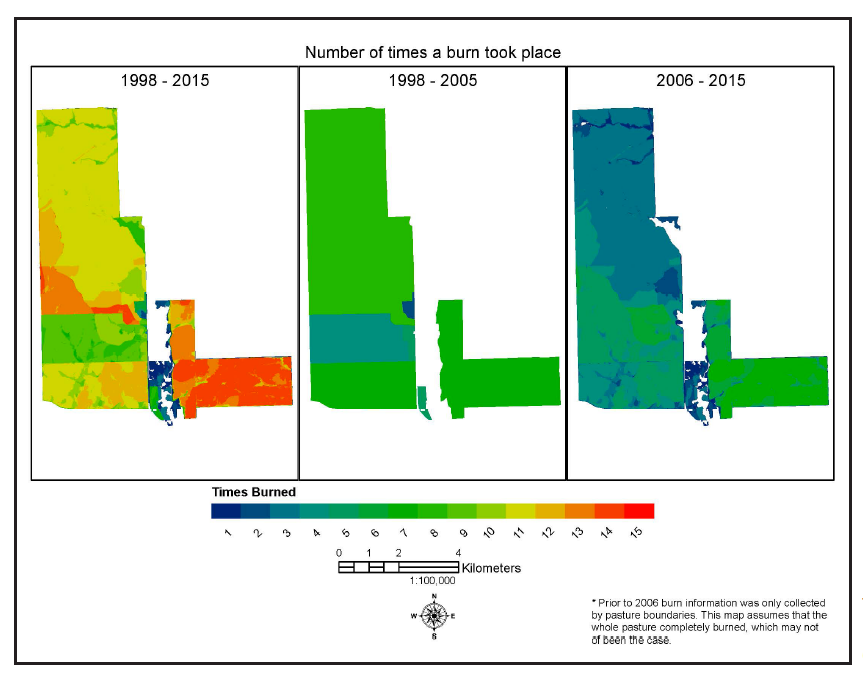
\includegraphics[width=0.75\textwidth]{figures/TAPR_Fire_mosaic.png}\caption[PBG at TAPR.]{Depiction of burn schedule in the Big Pasture Patch Burn Grazing
	system at TAPR.} \label{PBGatTAPR}
\end{figure*}

Patch-burn grazing research has typically occurred in southern grasslands and wetter climates. 
Lots of data has come out of the Konza Prairie Research Center in Kansas (\citep{powell2006} and the
Tallgrass Prairie Preserve in Oklahoma \citep{fuhlendorf2009}.
Positive effects on grassland ecosystems have been the norm in these studies. 
There have also been less numerous, but just as impactful, studies conducted in northern Great Plains displaying the positive aspects of patch burn grazing and specifically studying how the practice does not impact the drier landscapes via erosion, soil water content and soil temperature \citep{vermeire2005}.

Research has also focused on the use of livestock in a patch burn grazing system  \citep{fuhlendorf2001, vermeire2004, toombs2010, scasta2016}. 
The effects of fire and the interaction with livestock grazing has been studied and shown to increase productivity in forage and thus the vigor of cattle grazing within this system. 
Another studied aspect is seasonality with little effect difference on the cattle using the landscape \citep{vermeire2004}. 
This means that season of fire can be adjusted in terms of other management goals with no negative effects on herbivores.

\hypertarget{manage-for-system-processes}{%
\subsubsection{Manage for System Processes}\label{manage-for-system-processes}}

Overall, units need to focus on the enhancement of ecological resilience. 
The ideal way to naturally enhance ecological resilience is to increase the level of heterogeneity within on the landscape.
Heterogeneity creates diversity which is important to encourage diversity of resources. 
Diverse allows the ecosystem to respond to a variety of negative pressures.

\hypertarget{key-uncertainties-and-data-gaps}{%
	\subsection{Key Uncertainties and Data
		Gaps}\label{key-uncertainties-and-data-gaps}}

\begin{itemize}
	\item Vegetation management plans
	\item Forage productivity data
\end{itemize}

\hypertarget{vegetation-management-plans}{%
	\subsubsection{Vegetation Management
		Plans}\label{vegetation-management-plans}}

A common issue communicated by management staff was they feel they do not have written plans to manage for vegetation within their units. 
A definite focus of the NPS is wildlife as this is the charismatic entity that most visitors can connect with. 
At many units within this study, there are several plans in place for the mammalian species within their
management boundaries (bison, bighorn sheep, prairie dogs, black footed ferrets, etc.) 
There is data on vegetative communities collected both by the units themselves and I\&M surveyors, but, without management plans, there are no short-term or long-term specific goals to use these data to achieve. 
For example, species specific plans give numbers of animals or seral states to achieve through stocking rate, but vegetation is a more difficult resource to establish thresholds based on its dynamic nature especially in consideration of natural disturbances in a grassland ecosystem. 
The future of management could be defined by the creation of an ecosystem plan rather than a continuance of resource specific plans.
This could be the beginning of a new way of managing an ecosystem for all its parts rather than defining goals by one resource at a time.
Vegetation sampling appears to currently be the charge of the Northern Great Plains Network Inventory and Monitoring Program. 
An established monitoring protocol exists and is used at plots which were created across the units (Symstad et al. 2012). 
A depiction of the sampling plots is shown in Fig.~\ref{NGPNprotocol}.

\begin{figure*}[th]
	\centering
	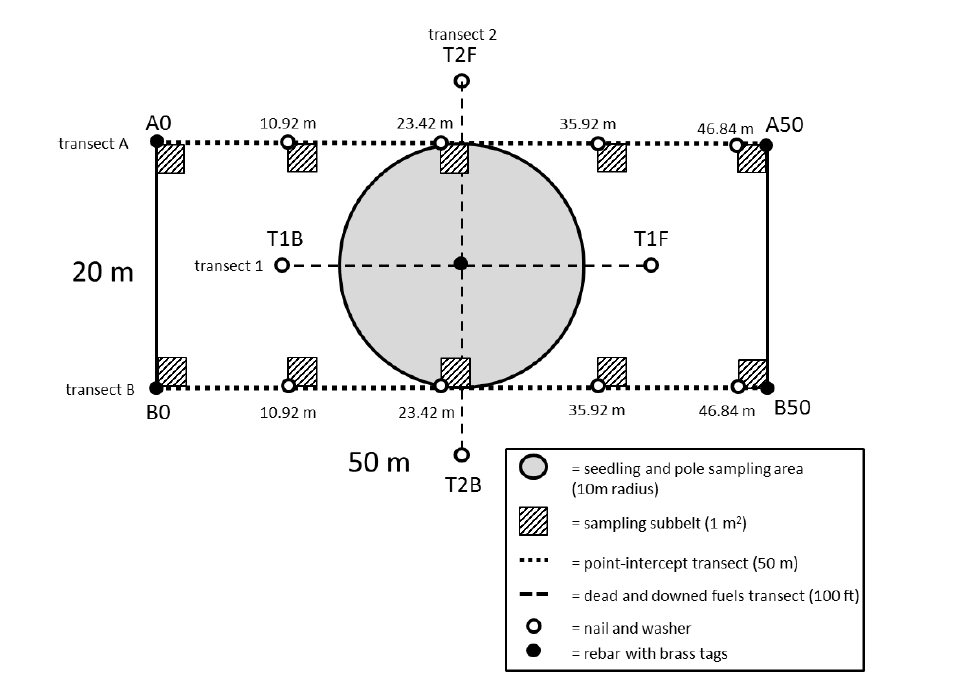
\includegraphics[width=0.75\textwidth]{figures/ngpsampling.png}\caption[NGPN Plant Community Composition Monitoring Protocol.]{NGPN Plant Community Composition Monitoring Protocol} \label{NGPNprotocol}
\end{figure*}

\hypertarget{forage-productivity-data}{%
	\subsubsection{Forage Productivity
		Data}\label{forage-productivity-data}}

In order to create a coupled disturbance regime, the piece of data we believe is most needed is plant productivity data of the vegetative community. 
Knowing how productive the protected landscape is each year allows you to better understand what type of disturbance regime will most positively impact your ecosystem. 
Factors of disturbance that would be influenced by plant productivity data could include: stocking rate of managed herbivore populations, fire return intervals, spatial extent of both fire and grazing, season of fire, etc.

Vegetation data collected by park units is lacking significantly behind wildlife data on a year-to-year basis. 
Vegetation data seems to be the focus of inventory and monitoring (I\&M) networks across the country.
This form of data collection is beneficial, but is also a standardized methodology not suited to alteration for varying unit-specific goals. 
It is also, as it was designed, monitoring focused. 
This means that it has no use as evidence of the effect of different management actions. 
I\&M collects species composition, forage cover etc., but not plant productivity data.

Studies that have used plant productivity as a means to determine disturbance rates have typically used NRCS Web Soil Survey data related to ecological site descriptions. 
Ecological site descriptions can be a very helpful metric, but climate and landscape topography are extremely variable in units within this region. 
This variety encourages the need for landscape specific data meaning data collected on site in specific locations of the unit. 
With this site specific data, the most positive disturbance regime is designed.

A unit that has prioritized the need for plant productivity data is BADL. 
Researchers are collecting data to better understand grazing resources and vegetative health \citep{symstad2016}. 
The key piece of this project is they are focusing on the integration of vegetation health and thinking of the vegetation as a grazing resource.
This is the beginning of systems thinking and as per our objectives, aligns with our hopes for recommended management changes. 
We recommend collecting plant productivity data and as this study is already established in the region, similar data collection methods could be transferred to other units in this study.

Data collection methods include aspects of a range assessment. 
Caged exclosures and the analysis of clipped vegetative material beget information on how productive the landscape is without grazing pressure.
This illuminates the amount of forage the landscape can produce and thus helps to determine how much the landscape can provide for grazers. 
This can also show how much of the landscape can be burned in order to maintain enough forage for the amount of grazers chosen. 
This is why coupling the two disturbances is important, it is necessary to consider both in order to best benefit the landscape and the broad range of resources that make up and depend on it.

Clipping vegetative material and then weighing this materials for mass productivity is a standard weigh to understand productive capability of a landscape \citep{mcnaughton1996}. 
The input of staff to accomplish these data collection methods may be cumbersome to achieve in some instances, so we propose altering the methodology from this study slightly if implementation were to take place across the Midwest region.
In the BADL study, they clip and sort the vegetation by species in order to get species composition across the landscape. 
Although this is beneficial information for forage selection by herbivores, when just looking at plant productivity, the time taken for sorting is unnecessary. 
Focusing on a species perspective versus a systems perspective, the individual species of vegetation does not matter as much as the overall production capability of the landscape.